
\Chapter{
    ``For you are dust, and to dust shall you return.''
\\[5pt]
\rightline{{\rm --- The book of genesis 3:19}}
}{The Roles and Physics of Aeolian Dust}

The first part of this chapter will delve further into the topic of dust, focusing on how dust impacts climate and the interrelationship between climate and dust, and conversely placing dust deposits as an important archive of past environmental change. Then \Cref{sec:dust_modelling} will look into how dust models works, and outline the physical processes behind dust emission, transport and deposition, which lay at the core of any dust model. Concluding this section will be a summary of what is the current challenges of advancing dust modelling. The second part of this chapter will focus on East Asian region specifically. Beginning with describing the location and characteristics of the main sources regions, followed by an overview meteorological conditions that responsible for producing dust events and the climatology of dust events. \textbf{In sec xxx} will describe the main modes of variability in circulation namely the arctic occilation the east asian winter monsoon. 

\section{Dust's role in the climate system}\label{seq:physics_of_dust}
\begin{figure}[htpb]
    \centering
    \includegraphics[width=\textwidth]{texfiles/figs/Desert_distrubtion.PNG}
    \caption{Earth's distribution of arid regions, adopted from \textcite{williams_climate_2014}}
    \label{fig:desert_distrubtion}
\end{figure}
Aeolian dust is one the most abundant aerosol species in the atmosphere and accounts for the majority of the total atmospheric aerosol mass. Aeolian dust referrers to dust that is emitted and transported by winds and the word aeolian stem from the Greek god Aeolus which in Greek mythology is the keeper of the winds. Around 1/3 of the earth surface is covered by deserts, that is regions where the precipitation is too low and evaporation too high to allow plants to grow \parencite{williams_climate_2014}.
As shown in \Cref{fig:desert_distrubtion} a large portion of the arid regions are located between 20\degree - 40\degree north/south, this region is known as the dust belt. The dust belt coincides with the descending part of the Hadley circulation. The descending motion creates a very stable atmosphere that suppresses the formation of rainfall. 
Other areas that typically experience a very limited amount of rainfall are places that are situated in the rain shadow of the surrounding topography or far in the interior of the continents where there are no proximal sources of moisture.  
The main dust sources are found in regions such as the Sahara, Middle East and northwest China. 

The dry conditions produce loose soils that are easily erodible. Thus during periods of strong winds dust emissions are naturally produced and entrained into the atmosphere. Producing an estimated 2000Mt of atmospheric dust each year, with around 1500Mt being deposited on land and about 500Mt being deposited into the ocean \parencite{shao2011dust}.  If the dust gets entrained into the upper troposphere it can be transported by the winds for thousands of kilometres \parencite{yumimoto_elevated_2009}. While in the atmosphere the dust particles directly affect the transfer of radiation through the atmosphere. 
The smallest dust particles between 0.2-\SI{2}{\micro\metre}, that has a size around the same order as the wavelength of visible light are the most efficient at scattering incoming solar radiation back to space. Accordingly, the smallest particles have a cooling effect on climate. Conversely, the larger particles (> \SI{4}{\micro\metre}) produces has a warming effect on climate due to their larger size which makes them efficient at absorbing terrestrial longwave radiation \parencite{choobari2014global}.
The lifetime of the dust aerosol is also strongly dependent on particle size \parencite{mahowald2014size}. Constraining the direct radiative effect of dust aerosols requires thus both getting the magnitude and size distribution of the emitted dust correct \parencite{adebiyi2020dust}.

% \subsubsection{Indirect radiative effect of dust: the impact dust of on clouds}
In the atmosphere dust also interact with clouds by acting \acrfull{in} and \acrfull{ccn} altering the microphysical properties of the clouds \parencite{lohmann2006sensitivity}. Dust aerosols in their unaltered state are usually hydrophobic and thus quite inefficient \acrshort{ccn}. However, during transport dust aerosols can acquire a coating of soluble material enhancing their ability as \acrshort{ccn} \todo{citation}. Dust aerosols have also been suggested to warm the clouds as dusty clouds have been observed to have a lower liquid water path compared to their dust-free counterpart \parencite{huang2006satellite}, this effect is known as the semi-direct effect. The semi-direct effect might play a significant role in inhibiting precipitation over the desert regions \parencite{shao2011dust}. Much of the uncertainty in the radiative impact of dust aerosols on clouds is due to how sensitive clouds are to even small changes in their microphysical properties (e.g. droplet size, droplet concentration and cloud phase). Dust aerosols have also been discovered to have an influence on tropical cyclones. Where tropical cyclones that intercepted as dust cloud was found to be significantly weaker after passing through the dust cloud. Due to the increase in \acrshort{ccn} caused by the dust plume slowed the rate of converting cloud drops into precipitation affecting the amount and distribution of latent heat \parencite{rosenfeld2011pollution}.  

There is a growing amount of evidence on the impact of dust deposition on ecosystems. In particular for the ocean biomass productivity where dust is an important source of iron. In the ocean iron is a limiting factor for phytoplankton production which is responsible for nearly half of the annual \ch{CO2} exchange between the atmosphere and the ocean and the majority of carbon sequestration on geological time scales \parencite{shao2011dust}. Moreover, the impact of dust is not limited to ocean productivity, African dust has been found to be an important source of nutrients for the Amazon rainforest. The productivity of the Amazon rainforest is constrained by the availability of phosphorus. \textcite{yu2015fertilizing} estimated about 0.022 Tg of phosphorus is brought to be Amazon through deposition of African dust each year, which is comparable to the amount washed out by rainfall. Model estimates of dust variability during the 20th century showed that increased dust deposition to the ocean and the corresponding boost of ocean productivity has caused an additional 4ppm of \ch{CO2} to be taken up by the ocean. However regional shifts in precipitation and temperature due to desert dust changes caused a similar decrease of 6ppm \ch{CO2} in the terrestrial biosphere carbon sink \parencite{mahowald2010observed}. Demonstrating that determining the net influence of dust on the biosphere and ultimately the carbon cycle is not straightforward.
\subsection{Dust as a climate archive}
Dust emission fluxes, size distribution and mineralogical composition are all strongly influenced by the wind speed, soil moisture and vegetation cover, and therefore indirectly modulating dust's role in the climate system. 
These climatic variables have experienced large changes throughout the history of Earth's climate and more pressingly are expected to change under the current anthropogenic global warming. Dust transport is if affected by changes in the atmospheric circulation and wet deposition by precipitation changes. There is consequently,
a potential for feedbacks involving dust and climate change. Thus dust archives are a window into the past from which the interconnections between climate and dust can be studied to help us understand the role dust will play in near future climate. 

Variations in \acrfull{mar}, particle size distribution have been used to reconstruct changes in large scale-circulation patterns and dust transport pathways, climatic changes in dust source and deposition areas and providing constraints for model reconstructions of past global climate states. Terrestrial deposits of aeolian dust or loess occupy large areas of North America, China, Central Asia and Europe with the most prominent Loess deposits located over \acrfull{clp}. In addition to loess, aeolian dust is also found in ice cores and deep sea records. One of the best documented features in the dust record is the variation in \acrfull{mar} between the glacial and interglacial periods. During glacial stages, the earth experienced increased dust loading. Findings from the dust records suggest that the high latitude dust loading were up to 25 times the present value and around two times at the lower latitude \parencite{shao2011dust}.     

       
%However current climate models struggles with reproducing many of the effects aeolian dust has on climate, due to their inability to accurately simulate the important dust processes such as dust emissions, transport and deposition \parencite{adebiyi2020dust}. 
\subsection{Dust modelling and observations}\label{sec:dust_modelling}
% Here I could write something about the historical context. 

The important role of dust in the climate system as pointed out in the previous section have inspired researchers across the scientific disciplines to put considerable efforts towards developing global and regional dust models. The field of dust modelling started to take off in the early 1990s when scientist realised that aerosols including dust were responsible for a large fraction of the uncertainties in the climate models due to the difficulties in determining the aerosol radiative effect \parencite{tegen1996influence}. Models have improved since then, and current state of the art models are able to reproduce large scale patterns of atmospheric dust load \todo{citation}. 
However, uncertainties in the description of
source areas and processes controlling dust emission and deposition produce a large spread in simulated dust fluxes \parencite{huneeus2011global}. This section provides an overview of the parameterisations of dust emissions, transport and deposition processes used in current dust models. The last part of this chapter will discuss some of the main discrepancies and uncertainties of current dust models.
% This motivated major efforts towards developing global dust models \parencite{dust_dist_Ginoux2001,zender2003mineral}.
%With the increased model resolution and further improvement of the model physics the global dust models has not only been used simulate time averaged dust features but also to study regional dust transport \parencite{zhao2006simulated} and studies of individual dust events. 

%Still current dust models are not able to adequately represent all the aspects of dust cycle, due to the computational complexity, lack of knowledge or limited observational constraints. The aim of this section is to describe how the different processes related to dust mobilisation, transport and deposition that are included in common dust models in use today and the main challenges and uncertainties related to these processes.      


%Most dust models are integrated systems  that are coupled to an atmospheric model, also called online dust models. However offline dust models also exist, these models relies on an external input data, commonly atmospheric reanalysis to provide the required atmospheric variables. The disadvantage of an offline is that new meteorological fields are only available at the temporal resolution of the input data, which is typically on the order hours. Whereas an online model the meteorological field would be updated at every model time step which depending on the use case could be on the order of minutes. On the other hand offline models are typically much faster to run as they do not have to calculate all the different atmospheric variables at each time step.           

\subsubsection{Dust emissions}\label{sec:dust_emission_modelling}
% dust emission is controlled by saltating sand particles which convey momentum of the wind flow to, and cast out, the finest dust particles lying in the bed
% the rich clay content, e.g., >20%, creates soil aggregates and clods so as to effectively depress sand saltation as well as dust emission 
%In general, three dust emission mechanisms are distinguished (Shao, 2008): direct aerodynamic entrainment/resuspension (Chepil, 1951, Chepil, 1965, Loosmore and Hunt, 2000), saltation bombardment/sandblasting (Chepil, 1965, Gillette et al., 1974, Shao et al., 1993, Alfaro et al., 1997, Eames and Dalziel, 2000) and disaggregation/auto-abrasion (Shao, 2008). 
Producing a realistic estimate of the spatial distribution of dust emission flux depends on the model realistically representing both surface properties and surface winds. Moreover, dust emissions are highly variable both spatially and temporally which means that the dust model has to account for emissions that occur on scales that are not explicitly resolved in the model.        

Dust is mobilised when the force exerted by the wind on the bare soil exceed the mobilisation threshold. The forces acting on a dust particle at rest is the aerodynamic force that exerts lift and gravitational and interparticle forces that tend to fix the particle the to ground. 
The strength aerodynamic force is governed by the amount of momentum transferred from the atmosphere to the surface which is described in terms of a friction velocity $u^*$ \parencite{ShaoYaping2008PaMo}.
\begin{equation}
    u_* = \sqrt{\tau/\rho}
\end{equation}
Here $\tau$ is the vertical component of the momentum flux and $\rho$ is the air density. The strength of the forces counteracting dust mobilisation primarily depends on the particle size. The effect of the interparticle forces decreases with larger particle size, but the larger particles are also heavier and therefore feel a stronger tug by gravity. Thus the particles that are most easily mobilised by the wind have a size corresponding to where the interparticle and gravitational forces are approximately equal in magnitude.     
The amount of force the wind has to exert on the dust particle to exceed the forces counteracting mobilisation is expressed by the threshold friction velocity. The expression obtained by \textcite{shao2000simple} is often used in the dust modelling community as it is relatively simple and straightforward. 
\begin{equation}
    u_{*t0}(d) = \sqrt{a_1 \left(\frac{\rho_p}{\rho_a}gd+\frac{a_2}{\rho_ad}\right)} 
\end{equation}
Here $a_1$ and the scaling constant for the inter particle forces, $a_2$  is assumed to be 0.0123 and \SI{3.0}{\kg\per\s\squared} respectively, which is  
according to \textcite{shao2000simple}, $\rho_p$ is the particle density and $\rho_a$ is the air density. 
The balance between the $u^*$ and $u^*_t$ is sensitive to several environmental factors such as weather (e.g. wind, precipitation and temperature), the soil composition, the soil moisture content, soil particle size distribution, vegetation converge and topography.  
\textbf{\begin{figure}[hptb]
    \centering
    \includegraphics[scale=0.7]{../figs/Threshold_friction_velocity.PNG}
    \caption{Threshold friction velocity $\mathbf{u^*}$ as a function of particle diameter. Measurements from wind tunnel experiments are represented by points, the lines represent different semi-empirical expression for the threshold friction velocity \parencite{kok2012physics}}.
    \label{fig:treshold_friction_velocity_ps}
\end{figure}}  
All these factors vary significantly both spatially and temporally making accurately calculating the threshold friction velocity difficult \todo{reference}. \Cref{fig:treshold_friction_velocity_ps} show the the threshold friction velocity as a function of particle diameter, the coloured lines represent the semi-empirical relations for $u^*_t$ described in \textcite{iversen1982saltation} (pink), \textcite{shao2000simple} (green) and \textcite{bagnold1941physics}. The semi-empirical relations and measurement seems to agree on a minimum in $u^*_t$ around in the range between  \SI{75}{\micro\metre} - \SI{100}{\micro\metre}. However, these particles are too heavy to be the subject of long-range suspension, rather they will soon after entrainment take on a ballistic trajectory. The impact from the large particle impacting the soil bed then eject smaller clay-sized dust particles from the soil bed, this process is called sandblasting. These smaller particles can be subjected to long-range transport. Sandblasting is the predominant process of dust emissions and minor processes are often neglected. 

There have been proposed several physics-based schemes for estimating the vertical dust \parencite{MB95_dust_emission,alfaro2001modeling,shao2004simplification}. The main distinction between the present schemes lay in how the particle size information is represented in the model. The schemes can be divided into either one of two categories, bulk and size resolving dust emission schemes. The bulk schemes (e.g. the emission scheme by \parencite{MB95_dust_emission}) gives an estimate of the total dust flux $F$ but provide no information about particle size-resolved dust flux $F(d)$. The bulk dust flux is estimated by first calculating the horizontal saltation flux and then deriving the vertical flux from the horizontal dust flux \parencite{tegen2014numerical}. The scheme of \textcite{MB95_dust_emission} uses an empirical relation to relate saltation to the bulk dust flux by scaling the saltation flux by a proportionally constant that depends on the clay content. In bulk emissions schemes the particle size-resolved dust flux $F(d)$ is inferred by assuming the size distribution of the emitted dust particles $p_s(d)$. Based on the theory of brittle fragments \textcite{kok_scaling_2011} derived theoretical expression of the particle size distribution for dust particles between \SI{0.1}{\micro\metre} - \SI{20}{\micro\metre} which showed good agreement when compared against observed size distributions. The \textcite{kok_scaling_2011} size distribution has been included in current climate models and has been shown to improve the representation of dust aerosols when compared to observations \parencite{johnson2012global}. However, this particle size distribution only applies to dust emission events that are predominantly due to the fragmentation of soil aggregates \parencite{kok2012physics}.

% \begin{equation}\label{eq:shao04}
%     F(d_i;d_s)=c_y\eta \left[(1-\gamma)+\sigma_p\right](1+\sigma_m)\frac{Q(d_s)g}{u_*^2}
% \end{equation}

The particle size resolving schemes, e.g. \textcite{shao2004simplification}, can directly derive the size-resolved dust flux $F_(d_i)$. This scheme calculates the emissions of particles with a size $d_i$ generated by saltating particles of size $d_s$. However, the problem with these schemes is that they require knowing the parent soil particle size distribution and measurements of parent soil particle size distributions are not available on a global scale.

The surface roughness $z_0$ is another important parameter for estimating the dust emissions as it is required for calculating the friction velocity from the surface. The $z_0$ used in global and regional models contain information about the subgrid-scale topography and vegetation in order to reproduce realistic grid-scale winds. However, these roughnesses operate on different spatial scales than the physical processes involved in dust emissions \parencite{darmenova_development_2009}. Therefore some models employ a satellite-derived dataset of surface roughness to obtain roughness on scales relevant for aeolian processes . 
%Many of the environmental factors have been accounted for based on empirical relations derived from several wind tunnel experiments and field measurement campaigns conducted during the last 50 years. In recent years observations from earth observing satellites such as the MODIS satellites have become increasingly important. This allowed for global monitoring of dust storm and to derived necessary land-surface and atmospheric parameters for dust modelling.  



\subsubsection{Dust transport}
Dust transport is divided into several different regimes as illustrated in \Cref{fig:modes_of_dust_transport}, which mode of transport a dust particle is subjected is to predominately determined by the local wind speed and the size of the particle. Among the different modes of transport only long term suspensions in considered in current dust models. While dust particles with the longest lifetime in the atmosphere are less than \SI{20}{\micro\metre} there is a growing amount of evidence that under the right atmospheric conditions even giant dust particles larger than \SI{200}{\micro\metre} can be transported for thousands of kilometres \parencite{van2018mysterious}. In comparison with observation current dust models struggle with representing the coarse particle severely underestimating the lifetime of the coarse dust particles, while overestimating the fine mode \parencite{adebiyi2020dust}. 
\begin{figure}[htbp]
  \centering
  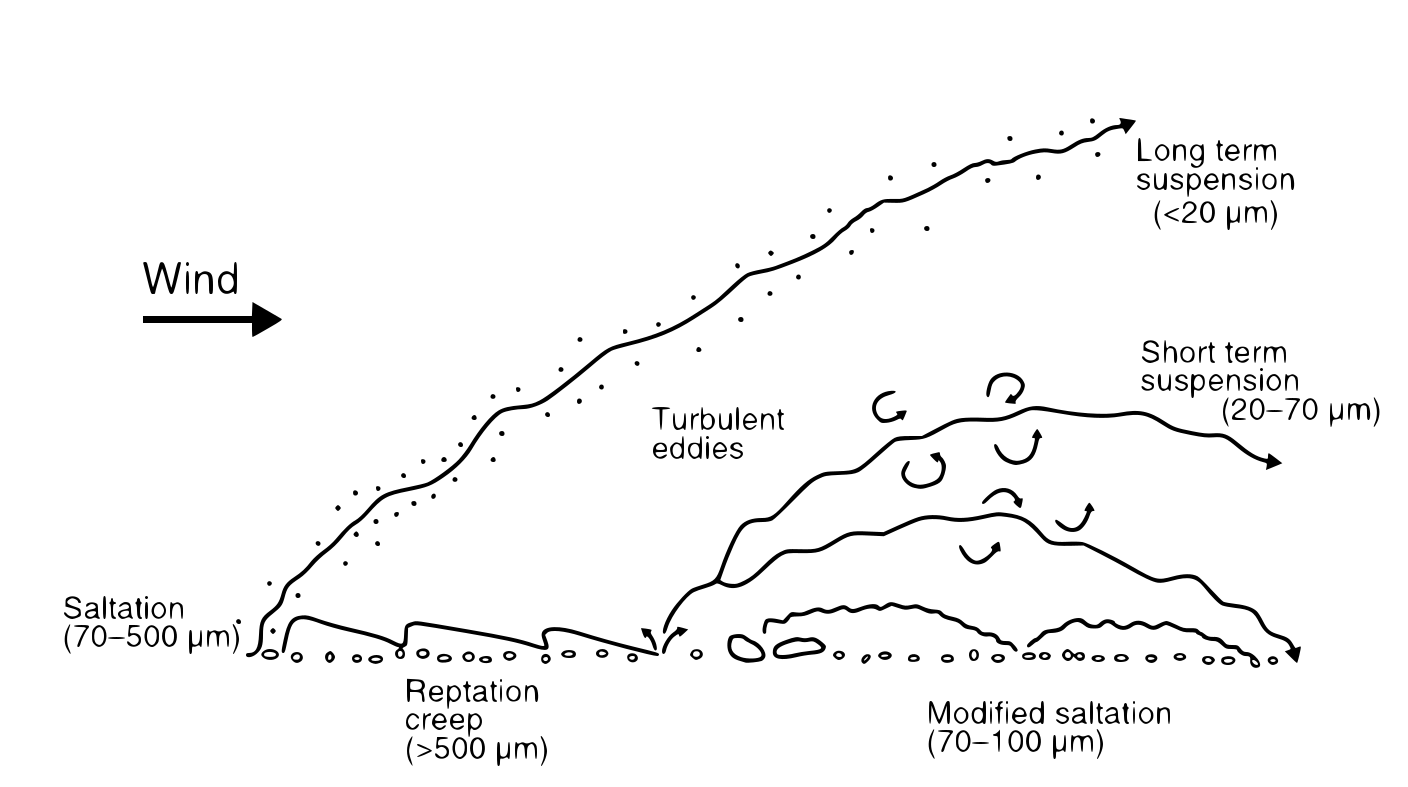
\includegraphics[draft=false,width = \textwidth]{texfiles/figs/aeolian_transport_Parsons_Abrahams.pdf}
  \caption{Different regimes of aeolian transport \parencite{nickling2009aeolian}}
  \label{fig:modes_of_dust_transport}
\end{figure}

Part of the reason why coarse dust is not well represented in current dust models is that they typically are non-spherical. Non-sphericity can have a significant impact on the settling velocity of the particle due to increased aerodynamic drag. The effect of the non-sphericity on settling velocity of dust particles was investigated by \textcite{mallios2020effects} and they found that non-spherical dust particles could remain significantly longer in the atmosphere compared to spherical particles of equivalent particle diameter. The non-sphericity of dust particles is not included in current dust models. Moreover, dust models cannot directly model the turbulent properties of the near-surface flow. The surface turbulence is import both important for the entrainment of coarse dust \parencite{klose2013large} and in facilitating the dust to stay aloft longer \parencite{ryder2013impact}. Electric charging of the dust particles counteracting the gravitational settling has also been proposed to affect the lifetime of the dust particles and is something that still remains unexplored in dust models.     

\subsubsection{Dust deposition}
Dust can be removed from the atmosphere either through dry or wet deposition. Dry deposition typically is the dominant processes close to the source region as there are still many large dust particles present. As the dust is transported further away from the source region the larger particles fall out and the dust size spectrum becomes narrower and the mode finer \parencite{does2016particle}. Dry deposition becomes less efficient at finer particle sizes and thus far from the source wet deposition is usually the dominating process \todo{citation}. There are two distinct routes a dust particle can be wet deposited, in-cloud or below-cloud scavenging: In-cloud scavenging the dust particles are rained out from the cloud through serving as \acrshort{ccn}s or \acrshort{in}s or by colliding with existing cloud particles. Below-cloud scavenging involves the dust particles being captured by falling hydrometeors. 

In dust models, the deposition is typically represented by a deposition velocity. For dry deposition, the predominant factors in determining the deposition velocity factors are the size of the dust particle and the density. Dry deposition is commonly modelled by a multi-layer resistance scheme. A widely used scheme used for modelling dry deposition is the two-layer resistance model of \parencite{slinn1982predictions}. The resistance model divides the atmosphere into two distinct layers; The quasi-laminar sublayer close to the ground which has a thickness on the order of centimetres and the constant flux layer above. In the quasi-laminar sublayer, Brownian diffusion and gravitational settling are the two main deposition processes. Within the constant flux layer turbulent motions and gravitational settling dominate. The gravitational settling velocity can be expressed by the modified stokes law of \parencite{slinn1982predictions}: 
\begin{equation}
    v_g = \frac{g\rho_p d_p^2 C_{cun}}{18\mu}
\end{equation}
Where $\rho_p$ and $d_p$ is the particle density and diameter, $\mu$ is the dynamic viscosity of air and $C_{cun}$ is the Cunningham slip-flow correction. The slip-flow correction accounts for the reduction in the drag force experienced by the smallest particles of sizes comparable to the mean free path of the molecules in air. The dry deposition velocity of a particle with a given size is given by a set of resistances, added to the settling velocity $v_g$:
\begin{equation}\label{eq:drydep_resistance}
    v_d=[r_a + r_b + r_a r_b v_g]^{-1} + v_g
\end{equation}
Here the $r_a$ represent the aerodynamic resistance, operating the constant flux layer and $r_b$ represent the resistance in the  surface layer quasi-laminar. There has be relatively few theoretical developments since the work of \textcite{slinn1982predictions} even though this model has be shown to well reproduce the dependence of $v_d$ on particle size \todo{reference}, it does not differentiate the deposition velocity between different surfaces \parencite{shao2011dust}. The difference in deposition rate between different surfaces is expected to be quite large \todo{reference}. 

The processes involved in wet deposition are complex and not well understood \todo{citation}. Between below-cloud and in-cloud scavenging below-cloud scavenging is the simpler and better studied process.
There are two mechanisms that reduce the below-cloud scavenging efficiency: (1) fine dust particles with diameters less than \SI{2}{\micro\metre} tend to follow the streamlines and flow around the droplet and (2) the dust particles might bounce off after colliding with the droplet. 
Accordingly, below-cloud scavenging is typically most efficient for the larger dust particles \todo{reference}.
Currently data is lacking for determining  probability of retention during the collision with the droplet, hence this mechanism is not included in current dust deposition schemes \parencite{ShaoYaping2008PaMo}. Several schemes for estimating the below-cloud scavenging efficiency $\lambda$ of varying level of complexity have been developed. The more complex semi-empirical schemes explicitly calculate the collection efficiency $E(r,R)$ which is a function of both the droplet and dust particle radius \parencite{seinfeld1998atmospheric, ShaoYaping2008PaMo}. 
Thus producing a collection efficiency for each dust particle droplet pair, however $E(r,R)$ require knowing droplet size distribution which is not always available in the model. Empirical below cloud scavenging schemes directly relate scavenging coefficient to the precipitation rate \parencite{brandt2002modelling} and thus avoiding the uncertainties in determining  the collection efficiency \parencite{jung2006intercomparison}. The empirical scheme of \parencite{laakso2003ultrafine} also included a dependence of dust particle size for the scavenging efficiency. 
\begin{figure}[htpb]
    \centering
    \includegraphics[draft=False,scale=.5]{texfiles/figs/Scavenging.PNG}
    \caption{Comparison of below cloud scavenging coefficients for three different below-cloud scavenging schemes; $\lambda_1$ \textcite{jung2006intercomparison},$\lambda_2$ \textcite{brandt2002modelling} and $\lambda_3$ \textcite{laakso2003ultrafine}. Adopted from \textcite{jung2006intercomparison}}
    \label{fig:scavenging}
\end{figure}
The below-cloud scavenging efficiency does primarily depend on the size and terminal velocity of the droplet relative to the dust particle. Typically the droplet size is inferred from the precipitation rate 
Accurately modelling dust deposition is challenging due to the difficulties of accurately predicting how the dust particle will behave during transport as discussed previously. 
The dust deposition parameterization depends on particle size and density as well
as on relevant meteorological quantities.

The processes involved in wet deposition are complex and not well understood \todo{citation}.



%\section{Lagrangian Models}
%An advantage with Lagrangian models is that they essentially do not exhibit numerical diffusion, except for errors related to interpolating the meteorological input data to the particle positions, in contrast to Eulerian models which often suffer from numerical diffusion \parencite{cassiani_offline_2016}. \textcite{cassiani_offline_2016} evaluated the offline FLEXPART-NorESM against the online tracer solver within NorESM and showed that the horizontal diffusion was around 10 times stronger for the online NorESM solver compared to the offline FLEXPART-NorESM. 

%An interesting possibility of LPDM is that they can be run can either be run forward or backwards in time, by simply switching the sign of the advection. Forward simulation, are a natural choice for studying the dispersion of tracers from known sources, for example the dispersion of nuclear fallout where you have one point source but an unknown number of receptors. While a forward simulation indicate where an atmospheric tracer will go, a backward simulation indicate where the tracer came from. Therefore backward simulations are useful for interpreting measurements of atmospheric trace substances and to establish relationships between the sources and their receptors.  



\section{East asian dust}

\subsection{Characterisation of East Asian dust sources and deposition areas}
The majority of the East Asian deserts are located in arid regions of Northern China and South east Mongolia. Situated in the interior of the Eurasian continent far removed from the moisture from the Pacific ocean and the prevention of south west transport by the mountains of the Tibetan plateau makes these regions exceptionally dry.  Together the East Asian desert regions makes up the second largest source of atmospheric dust aerosols \parencite{chen2017overview} with an estimated annual emissions of \textbf{XX}Mt - \textbf{XX} \todo{Find reference}. 

\todo{Need a nice map of dust sources maybe Hui can provide?}

In therms of the morphology and composition of the surface soil, the East Asian desert can separated into two classes gobi-desert and sand desert \parencite{xuan2002characterization}. Gobi characterise regions consisting of pebbles, gravel and rock debris and gobi-desert then refers to an area consisting of interluding regions of sandy deserts, gobis and grassland. Gobi and gobi-deserts are mainly found in the northern region of the Inner Mongolia plateau and the southern part of Mongolia, this whole region is commonly referred to as the Gobi desert. Sand deserts primarily consists of loose sand and the largest sand desert in the regions are the Taklamakan desert located in the Tarim basin and the   

\subsection{Atmospheric circulation in East Asia}
The most prominent feature of the atmospheric circulation in the East Asian region is the monsoon system. A monsoon wind system is one that seasonally changes direction, blowing from one direction in the summer and in the opposite direction in the winter. The primary driver of the East Asian monsoon system is the temperature contrast between the land and ocean. During the winter months the land is generally colder than the ocean where the main heating source is located over the equatorial western pacific. The convection associated with the heating drives a large scale meridional overturning circulation where the airmasses rises over the ocean and then subsides over the Siberian region. Creating a persistent high pressure system over Siberia during the winter. This circulation is the East Asian Winter Monsoon (EAWM). During the East Asian Summer Monsoon (EASM) the situation is reversed. In the summer the land is much warmer than the ocean, the heating on land drives strong convection which creates a persistent low pressure at the surface. The low pressure drags moist air from the ocean inland. Upon reaching the Tibetan Plateau the moist air is lifted and consequently cooled which causes the water vapor to condense resulting in intense precipitation. 

In following section will describe the EAWM and EASM circulation and how they are influenced by ...   

\subsection{East Asian Winter Monsoon}
\begin{figure}[htpb]
    \centering
    \includegraphics[width=\textwidth]{texfiles/figs/climatology_1999-2019.pdf}
    \caption{The 20 year average of winter (DJF)  and spring (MAM) circulation from ERA5. (a) Winter and (b) spring \acrshort{mslp} and 850hPa winds climatology. (c) Winter and (b) spring 500hPa geopotential height and winds. (e) winter and (f) spring 200hPa geopotential height and windspeed.}
    \label{fig:clim_circulation}
\end{figure}
The EAWM dominates the climate in East Asia during winter months, December, January, February, and is closely related to the cold core of the Siberian High. The \acrshort{eawm} circulation is primarially driven by the temprature contrast between the relative cold and warm ocean. \acrshort{eawm} consist of 3 subcomponets which can be identified in \Cref{fig:clim_circulation}, at the surface the Siberian High and Alutian low, East Asian trough can be identified at the 500hPa level located around 120\degree E and 50\degree N  
\begin{figure}[htpb]
    \centering
    \includegraphics[width=\textwidth]{texfiles/figs/winter_MO_AO_composite.pdf}
    \caption{Circulation composite anomalies of 850hPa winds and mean sea level pressure for strong - weak winter monsoon years and negative - positive winter AO. (a) and (b) is the DJF anomalies and (c) - (d) is MAM anomilies in the following spring}
    \label{fig:mo_ao_composite}
\end{figure}

\subsection{The impact of Arctic Oscillation on the East Asian Climate}
\begin{figure}[htpb]
    \centering
    \includegraphics[width=\textwidth]{texfiles/figs/EOF_AO_NAO.pdf}
    \caption{The spatial correlation of the leading EOF of 1000hPa geopotential height (a) representing the \acrshort{ao}. (b)  spatial correlation of the leading \acrshort{eof}  of SLP anomalies over the Atlantic sector, 20\degree-80\degree N, 90\degree W-40\degree, representing the \acrshort{nao}.}
    \label{fig:EOF_NAO_AO}
\end{figure}
The \acrfull{ao} is represented by the leading EOF of the 1000hPa geopotential height poleward of 20 \degree N \parencite{thompson1998arctic}. In it's structure it resembles the \acrfull{nao} except being more zonally symetric in structure. The AO has been shown to have a significant impact on the \acrshort{eawm} where negative winter AO is usually associated with a stronger winter monsoon and vice versa. Cold events are also found to be more frequent over East Asia during negative AO conditions \parencite{he2017impact}. \textcite{wu2002winter} examined how the \acrshort{ao} influence the \acrshort{eawm} and found that the AO directly influence surface air temperature (SAT), \acrshort{mslp} and the East Asian Trough at 500 hPa over the region northwards of 35°N in East Asia rather than through its impact on the SH. The SH in comparison had more direct impact on the \acrshort{eawm} through influencing the \acrshort{mslp} and the northly wind along the east asian coast. However due to the how \acrshort{ao} suppresses the influence of the \acrshort{sh} on the higher latitudes, the influence of the \acrshort{sh} happens primarily southwards of 50\degree N over East Asia \parencite{wu2002winter}. 

\begin{figure}[htbp]
    \centering
    \includegraphics[width=\textwidth]{texfiles/figs/winter_MO_AO_composite_500h.pdf}
    \caption{Circulation composite anomalies of 500hPa winds and geopotential height for strong - weak winter monsoon years and negative - positive winter AO. (a) and (b) is the DJF anomalies and (c) - (d) is MAM anomilies in the following spring}
    \label{fig:mo_ao_composite_500hPa}
\end{figure}

\subsection{Characterisation of East Asian dust sources and deposition areas}
The majority of the East Asian deserts are located in arid regions of Northern China and South east Mongolia. Situated in the interior of the Eurasian continent far removed from the moisture from the Pacific ocean and the prevention of south west transport by the mountains of the Tibetan plateau makes these regions exceptionally dry.  Together the East Asian desert regions makes up the second largest source of atmospheric dust aerosols \parencite{chen2017overview} with an estimated annual emissions of \textbf{XX}Mt - \textbf{XX} \todo{Find reference}. 

\todo{Need a nice map of dust sources maybe Hui can provide?}

In therms of the morphology and composition of the surface soil, the East Asian desert can separated into two classes gobi-desert and sand desert \parencite{xuan2002characterization}. Gobi characterise regions consisting of pebbles, gravel and rock debris and gobi-desert then refers to an area consisting of interluding regions of sandy deserts, gobis and grassland. Gobi and gobi-deserts are mainly found in the northern region of the Inner Mongolia plateau and the southern part of Mongolia, this whole region is commonly referred to as the Gobi desert. Sand deserts primarily consists of loose sand and the largest sand desert in the regions are the Taklamakan desert located in the tarim basin and the    


\subsubsection{Dust storm climatology}
In the winter the desert regions are dominated by the cold \acrshort{sh} causing parts of the desert to be covered in snow and the soil to frozen. The frozen soil thaws in spring leaving the surface loose and prone to wind erosion. 
The majority of the dust events in East Asia occur during the spring months from March until May with half of the dust events occurring in April \parencite{sun2001spatial}. The dust storms are associated with cold air outbreaks which initiate the formation of the Mongolian cyclone and frontal systems. About 80 \% of the dust events are associated with an active Mongolian cyclone where as the remaining are caused by the passage of cold fronts \parencite{sun2001spatial}.
The number of cold air outbreaks occurring in spring is much influenced by the intensity and location of the jet stream. A strong jet stream inhibits air mass exchange between lower and higher latitudes whereas and confine the cold air to the high latitudes \parencite{wang2008variability}. There has been large decrease in the number of dust events in East Asia since 1980s which has been hypothesised to be the result of arctic amplification and weakened temperature gradients \parencite{liu2020impact}. 

% it has been known that there are three major motions of wind‐blown sand particles, i.e., creep, saltation, and suspension

% Except for dust storms in which the suspension motion is dominant, saltation plays a key role in the wind erosion process
\subsubsection{Deserts regions in East Asia}
The main desert regions in east Asia is the Gobi Desert, Taklamakan desert, Badain Jaran Desert, \todo{Need map} and the Mu Us Desert. The Taklamakan desert is located in the tarim basin is the second largest sand desert in the world. The desert is surrounded by tall mountain ranges on both sides which can mechanically lift dust veils into the upper tropshere \parencite{yumimoto_elevated_2009}.   There are difference in soil composition between the different deserts. Gobi Desert is a primarialy stone desert, compared to Badain Jaran and Taklamakan which both sandy desert. The Badain Jaran desert has the tallest sanddunes in the planet. 

%And, southwest of the plateau, the bottom of the Old Tarim Basin and Old Junggar Basin had also lifted to 1000 m elevation but still remained lower than the surrounding topography. The modern Tarim Basin and Junggar Basin are surrounded by the Altaj Mountains in the north, Tainshan Mountains in between, Tibetan Plateau in the south, Pumir Plateau in the west, and Mongolian Plateau and Kunlun Mountains in the east

%It is suggested that the source region in East Asia consists of two parts or systems: (i) the Mongolian Plateau dust source system, including deserts and gobi-deserts on the Mongolian Plateau and its southern extension—the Ordos Plateau and Alxa Plateau; and (ii) the Tarim Basin dust source system, including deserts and gobi-deserts in the Tarim Basin, Junggar Basin, and eastern vicinity.

%classified dust storms in East Asia into four types, among which the S (stationary) type and M (moving) type are basic ones. 80\% of their S type dust storms occurred over the Taklimakan Desert and vicinity, while 70\% of the M type originated over the gobi area and desert area of 90–105°E, i.e., the Mongolian Plateau and its southern extension.

\subsubsection{Gobi desert}


%Gravel covering the gobi surface can effect the dust emission both positively and negatively: gravel half-buried in sand (soil) surfaces decreases the effective wind shear force on the soil surface, resulting in stress partitioning (Nickling and Gillies, 2003), and a complete stony armor strongly depresses the aeolian motion of particles (Yi et al., 2002). 

%precipitation is rare in the gobi area, less than 50 mm yr−1 (Zhao, 1994), and is limited to the summer season so that the gobi surface becomes extremely dry in spring when the strong wind behind a cold front periodically blows through East Asia and is enhanced over the vast and flat gobi surface. As the surface wind speed often reaches 24–30 m s−1, or even higher, on the south Mongolian Plateau (Qian et al., 1997), strong dust storms occur in spite of the gravel armoring and the below 0°C air temperature. 

%Thousands of kilometers from the oceans and high above the sea level, the Mongolian climate is extremely dry, continental and cold.

%  It is also normal in Mongolia that the annual precipitation varies greatly from year to year. For example, the precipitation in Sainshand (44°52′N, 110°09′E) was 83 mm yr−1 in 1963 but, in the next year, it went up to 248 mm yr−1 (CMA, 1970). Such a great interannual change in precipitation means that, in drought years, severe dust storms occur even in the north mountain area. At the end of winter season, the south Siberian anti-cyclone named the ‘Siberian High’ becomes unstable and, in the following spring months, breaks down several times so that a succession of frontal systems traverses the country from northwest to southeast, resulting in strong surface wind, which is further strengthened over the vast and flat gobi surface. 

%In the Mongolian Plateau system and downwind vicinity, from northwest to southeast, the surface soil texture shows a coarse-to-fine trend: gobi gravel becomes desert sand, followed by silt and clay of the Loess Plateau. 

%A cold front passage in spring produces strong surface wind in both systems. Because of the difference in topography, northwest wind and northeast wind respectively prevail in the Mongolian Plateau system and the Tarim Basin system. 
\subsubsection{The Chinese Loess Plateau}
%On the Loess Plateau, the content of silt and clay in the surface soil is more than 90\% and the sand and gravel content is in totally lacking (Xiong and Li, 1990). Also, the annual mean precipitation is around 400 mm yr

%Loess Plateau is the center of a strong dust-fall region. Their chemical analysis of soil samples proves also that the Loess Plateau was formed by millions of years of dust deposition (Zhang, 1999).